\chapter{Research Method \label{ch:methodology}}
\chaptertoc

This chapter describes the research method used to investigate architecture recovery and C2A mapping. It defines the research design and the graph-based representation-learning design space, then describes the input signals, learning settings, and controlled-comparison logic used across the studies. It also presents the benchmark systems and evaluation protocol, including the sampling of labeled files and statistical analysis. Finally, it describes the additional cross-study evaluation design.
\section{Research Design \label{sec:research_design}}

This thesis combines method development with empirical evaluation. Each study develops and evaluates a graph-based representation learning method for architecture recovery or C2A mapping. The studies investigate what architectural information is carried by implementation signals, including dependency structure, project organization, and code content, and the system conditions under which these signals support architectural analysis. Comparisons with established baselines assess whether the resulting methods are competitive, whereas controlled comparisons between graph configurations, input representations, and learning mechanisms examine the contribution of each.

\subsection{Design Space\label{sec:design_space}}

Architecture recovery and mapping are studied through a common graph-based representation-learning framework. The choices investigated across the thesis define a design space with four dimensions: graph topology, relation modeling, input representation, and learning mechanism, summarized in Figure~\ref{fig:design_space}. These dimensions are analytically distinct but not always experimentally independent: adding a node type usually requires a new relation type to connect it to the rest of the graph.
 
Graph topology determines which software artifacts are represented as nodes. The simplest configuration contains only file nodes. Richer variants add folder nodes, one per directory, member nodes that aggregate the program elements contained in each file, or include both folder and member nodes together. Relation modeling determines how these nodes are connected. Static dependencies may be merged into a single relation or preserved as typed relations such as \emph{call}, \emph{import}, and \emph{inheritance}. Graphs containing additional artifact types also include organizational and containment meta-relations, such as folder-to-folder, folder-to-file, and file-to-member relations.
 
Input representation determines what information is available to the nodes before message passing. Nodes may start with learnable identity embeddings or with features derived from dependency structure, folder organization, or code content. These features range from token-based representations and structural encodings to pretrained contextual code embeddings.
 
The learning mechanism determines how these inputs and graph relations are used to learn file representations. The studies compare random-walk methods and graph neural networks, with learning objectives suited to recovery or mapping.

% \begin{figure}[!thb]
%     \centering
%     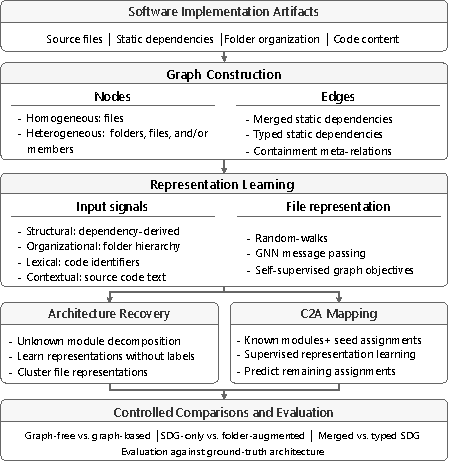
\includegraphics[width=1\textwidth]{figures/design_space.pdf}
%     \caption[Design space studied in the thesis.]{Design space studied across the thesis: graph configurations ranging from the SDG to heterogeneous folder-file-member graphs, initialized from structural, organizational, lexical, or contextual signals, and evaluated under unsupervised recovery and supervised mapping through controlled comparisons of relation modeling, graph structure, input representation, and learning mechanism.. \label{fig:design_space}}
% \end{figure}

\begin{figure}[!thb]
    \centering
    \begin{adjustbox}{max width=1\textwidth}
        % Included using % Included using % Included using \input{figures/design_space.tex}
\begingroup

% Header colors: edit only these two lines.
\colorlet{HeaderBackground}{gray!30}
\colorlet{HeaderText}{black}

% Panel arguments:
% left, top, right, bottom, header bottom, title
\newcommand{\figurepanel}[6]{%
    \path[fill=white] (#1,#2) rectangle (#3,#4);
    \path[headerfill] (#1,#2) rectangle (#3,#5);
    \draw[border] (#1,#2) rectangle (#3,#4);
    \draw[divider] (#1,#5) -- (#3,#5);
    \node[heading] at ({(#1+#3)/2},{(#2+#5)/2}) {#6};
}

\begin{tikzpicture}[
    x=0.9cm,
    y=1.2cm,
    font=\figurefont\small,
    text=black,
    headerfill/.style={fill=HeaderBackground, draw=none},
    heading/.style={
        text=HeaderText,
        font=\figurefont\normalsize\bfseries,
        align=center,
        inner sep=0pt
    },
    border/.style={draw=black!70, line width=0.6pt},
    divider/.style={draw=black!45, line width=0.5pt},
    connector/.style={draw=black!50, line width=0.8pt},
    arrow/.style={
        connector,
        -{Stealth[length=1.7mm,width=1.4mm]}
    },
    subheading/.style={
        font=\figurefont\small\selectfont,
        align=center,
        inner sep=0pt
    },
    content/.style={
        anchor=north west,
        align=left,
        inner sep=0pt
    }
]

% ============================================================
% Software implementation artifacts
% ============================================================

\figurepanel
    {0}{0}{13}{-1.15}{-0.55}
    {Software Implementation Artifacts}

\node[align=center,inner sep=0pt] at (6.50,-0.85) {%
    Source files
    \enspace$\vert$\enspace
    Static dependencies
    \enspace$\vert$\enspace
    Folder organization
    \enspace$\vert$\enspace
    Code content
};

\draw[arrow] (6.50,-1.15) -- (6.50,-1.45);

% ============================================================
% Graph construction
% ============================================================

\figurepanel
    {0}{-1.45}{13}{-3.95}{-2.00}
    {Graph Construction}

\node[subheading] at (3.25,-2.32) {Nodes};
\node[subheading] at (9.75,-2.32) {Edges};

\draw[divider] (0.25,-2.55) -- (6.25,-2.55);
\draw[divider] (6.75,-2.55) -- (12.75,-2.55);

\node[content,text width=6.00cm] at (0.25,-2.75) {%
    \strut- Homogeneous: files\\[3pt]
    - Heterogeneous: files/folders/members
};

\node[content,text width=6.00cm] at (6.75,-2.75) {%
    \strut- Merged static dependencies\\[3pt]
    - Typed static dependencies\\[3pt]
    - Containment meta-relations
};

\draw[arrow] (6.50,-3.95) -- (6.50,-4.25);

% ============================================================
% Representation learning
% ============================================================

\figurepanel
    {0}{-4.25}{13}{-7.15}{-4.80}
    {Representation Learning}

\node[subheading] at (3.25,-5.12) {Input representation};
\node[subheading] at (9.75,-5.12) {Learning mechanism};

\draw[divider] (0.25,-5.35) -- (6.25,-5.35);
\draw[divider] (6.75,-5.35) -- (12.75,-5.35);

\node[content,text width=6.00cm] at (0.25,-5.55) {%
    \strut- Structural: dependency-derived\\[3pt]
    - Organizational: folder hierarchy\\[3pt]
    - Lexical: code identifiers\\[3pt]
    - Contextual: source code text
};

\node[content,text width=6.00cm] at (6.75,-5.55) {%
    \strut- Random-walks\\[3pt]
    - GNN message passing\\[3pt]
    - Self-supervised graph objectives
};

% Split into the two downstream tasks.
\draw[connector] (6.50,-7.15) -- (6.50,-7.30);
\draw[arrow] (6.50,-7.30) -| (3.175,-7.55);
\draw[arrow] (6.50,-7.30) -| (9.825,-7.55);

% ============================================================
% Architecture recovery
% ============================================================

\figurepanel
    {0}{-7.55}{6.35}{-9.55}{-8.10}
    {Architecture Recovery}

\node[content,text width=5.95cm] at (0.20,-8.32) {%
    \strut- Unknown module decomposition\\[3pt]
    - Learn representations without labels\\[3pt]
    - Cluster file representations
};

% ============================================================
% Code-to-architecture mapping
% ============================================================

\figurepanel
    {6.65}{-7.55}{13}{-9.55}{-8.10}
    {C2A Mapping}

\node[content,text width=5.95cm] at (6.85,-8.32) {%
    \strut- Known modules + seed assignments\\[3pt]
    - Supervised representation learning\\[3pt]
    - Predict remaining assignments
};

% Merge the two task branches.
\draw[connector]
    (3.175,-9.55) -- (3.175,-9.70)
    -- (9.825,-9.70) -- (9.825,-9.55);

\draw[arrow] (6.50,-9.70) -- (6.50,-9.95);

% ============================================================
% Controlled comparisons and evaluation
% ============================================================

\figurepanel
    {0}{-9.95}{13}{-11.75}{-10.50}
    {Controlled Comparisons and Evaluation}

\node[align=center,inner sep=0pt] at (6.50,-10.95) {%
    Graph-free vs.\ graph-based
    \,$\vert$\,
    SDG-only vs.\ folder-augmented
    \,$\vert$\,
    Merged vs.\ typed SDG
};

\node[
    align=center,
    inner sep=0pt,
    font=\figurefont\small,
] at (6.50,-11.45)
    {Evaluation against ground-truth architecture};

\end{tikzpicture}
\endgroup
\begingroup

% Header colors: edit only these two lines.
\colorlet{HeaderBackground}{gray!30}
\colorlet{HeaderText}{black}

% Panel arguments:
% left, top, right, bottom, header bottom, title
\newcommand{\figurepanel}[6]{%
    \path[fill=white] (#1,#2) rectangle (#3,#4);
    \path[headerfill] (#1,#2) rectangle (#3,#5);
    \draw[border] (#1,#2) rectangle (#3,#4);
    \draw[divider] (#1,#5) -- (#3,#5);
    \node[heading] at ({(#1+#3)/2},{(#2+#5)/2}) {#6};
}

\begin{tikzpicture}[
    x=0.9cm,
    y=1.2cm,
    font=\figurefont\small,
    text=black,
    headerfill/.style={fill=HeaderBackground, draw=none},
    heading/.style={
        text=HeaderText,
        font=\figurefont\normalsize\bfseries,
        align=center,
        inner sep=0pt
    },
    border/.style={draw=black!70, line width=0.6pt},
    divider/.style={draw=black!45, line width=0.5pt},
    connector/.style={draw=black!50, line width=0.8pt},
    arrow/.style={
        connector,
        -{Stealth[length=1.7mm,width=1.4mm]}
    },
    subheading/.style={
        font=\figurefont\small\selectfont,
        align=center,
        inner sep=0pt
    },
    content/.style={
        anchor=north west,
        align=left,
        inner sep=0pt
    }
]

% ============================================================
% Software implementation artifacts
% ============================================================

\figurepanel
    {0}{0}{13}{-1.15}{-0.55}
    {Software Implementation Artifacts}

\node[align=center,inner sep=0pt] at (6.50,-0.85) {%
    Source files
    \enspace$\vert$\enspace
    Static dependencies
    \enspace$\vert$\enspace
    Folder organization
    \enspace$\vert$\enspace
    Code content
};

\draw[arrow] (6.50,-1.15) -- (6.50,-1.45);

% ============================================================
% Graph construction
% ============================================================

\figurepanel
    {0}{-1.45}{13}{-3.95}{-2.00}
    {Graph Construction}

\node[subheading] at (3.25,-2.32) {Nodes};
\node[subheading] at (9.75,-2.32) {Edges};

\draw[divider] (0.25,-2.55) -- (6.25,-2.55);
\draw[divider] (6.75,-2.55) -- (12.75,-2.55);

\node[content,text width=6.00cm] at (0.25,-2.75) {%
    \strut- Homogeneous: files\\[3pt]
    - Heterogeneous: files/folders/members
};

\node[content,text width=6.00cm] at (6.75,-2.75) {%
    \strut- Merged static dependencies\\[3pt]
    - Typed static dependencies\\[3pt]
    - Containment meta-relations
};

\draw[arrow] (6.50,-3.95) -- (6.50,-4.25);

% ============================================================
% Representation learning
% ============================================================

\figurepanel
    {0}{-4.25}{13}{-7.15}{-4.80}
    {Representation Learning}

\node[subheading] at (3.25,-5.12) {Input representation};
\node[subheading] at (9.75,-5.12) {Learning mechanism};

\draw[divider] (0.25,-5.35) -- (6.25,-5.35);
\draw[divider] (6.75,-5.35) -- (12.75,-5.35);

\node[content,text width=6.00cm] at (0.25,-5.55) {%
    \strut- Structural: dependency-derived\\[3pt]
    - Organizational: folder hierarchy\\[3pt]
    - Lexical: code identifiers\\[3pt]
    - Contextual: source code text
};

\node[content,text width=6.00cm] at (6.75,-5.55) {%
    \strut- Random-walks\\[3pt]
    - GNN message passing\\[3pt]
    - Self-supervised graph objectives
};

% Split into the two downstream tasks.
\draw[connector] (6.50,-7.15) -- (6.50,-7.30);
\draw[arrow] (6.50,-7.30) -| (3.175,-7.55);
\draw[arrow] (6.50,-7.30) -| (9.825,-7.55);

% ============================================================
% Architecture recovery
% ============================================================

\figurepanel
    {0}{-7.55}{6.35}{-9.55}{-8.10}
    {Architecture Recovery}

\node[content,text width=5.95cm] at (0.20,-8.32) {%
    \strut- Unknown module decomposition\\[3pt]
    - Learn representations without labels\\[3pt]
    - Cluster file representations
};

% ============================================================
% Code-to-architecture mapping
% ============================================================

\figurepanel
    {6.65}{-7.55}{13}{-9.55}{-8.10}
    {C2A Mapping}

\node[content,text width=5.95cm] at (6.85,-8.32) {%
    \strut- Known modules + seed assignments\\[3pt]
    - Supervised representation learning\\[3pt]
    - Predict remaining assignments
};

% Merge the two task branches.
\draw[connector]
    (3.175,-9.55) -- (3.175,-9.70)
    -- (9.825,-9.70) -- (9.825,-9.55);

\draw[arrow] (6.50,-9.70) -- (6.50,-9.95);

% ============================================================
% Controlled comparisons and evaluation
% ============================================================

\figurepanel
    {0}{-9.95}{13}{-11.75}{-10.50}
    {Controlled Comparisons and Evaluation}

\node[align=center,inner sep=0pt] at (6.50,-10.95) {%
    Graph-free vs.\ graph-based
    \,$\vert$\,
    SDG-only vs.\ folder-augmented
    \,$\vert$\,
    Merged vs.\ typed SDG
};

\node[
    align=center,
    inner sep=0pt,
    font=\figurefont\small,
] at (6.50,-11.45)
    {Evaluation against ground-truth architecture};

\end{tikzpicture}
\endgroup
\begingroup

% Header colors: edit only these two lines.
\colorlet{HeaderBackground}{gray!30}
\colorlet{HeaderText}{black}

% Panel arguments:
% left, top, right, bottom, header bottom, title
\newcommand{\figurepanel}[6]{%
    \path[fill=white] (#1,#2) rectangle (#3,#4);
    \path[headerfill] (#1,#2) rectangle (#3,#5);
    \draw[border] (#1,#2) rectangle (#3,#4);
    \draw[divider] (#1,#5) -- (#3,#5);
    \node[heading] at ({(#1+#3)/2},{(#2+#5)/2}) {#6};
}

\begin{tikzpicture}[
    x=0.9cm,
    y=1.2cm,
    font=\figurefont\small,
    text=black,
    headerfill/.style={fill=HeaderBackground, draw=none},
    heading/.style={
        text=HeaderText,
        font=\figurefont\normalsize\bfseries,
        align=center,
        inner sep=0pt
    },
    border/.style={draw=black!70, line width=0.6pt},
    divider/.style={draw=black!45, line width=0.5pt},
    connector/.style={draw=black!50, line width=0.8pt},
    arrow/.style={
        connector,
        -{Stealth[length=1.7mm,width=1.4mm]}
    },
    subheading/.style={
        font=\figurefont\small\selectfont,
        align=center,
        inner sep=0pt
    },
    content/.style={
        anchor=north west,
        align=left,
        inner sep=0pt
    }
]

% ============================================================
% Software implementation artifacts
% ============================================================

\figurepanel
    {0}{0}{13}{-1.15}{-0.55}
    {Software Implementation Artifacts}

\node[align=center,inner sep=0pt] at (6.50,-0.85) {%
    Source files
    \enspace$\vert$\enspace
    Static dependencies
    \enspace$\vert$\enspace
    Folder organization
    \enspace$\vert$\enspace
    Code content
};

\draw[arrow] (6.50,-1.15) -- (6.50,-1.45);

% ============================================================
% Graph construction
% ============================================================

\figurepanel
    {0}{-1.45}{13}{-3.95}{-2.00}
    {Graph Construction}

\node[subheading] at (3.25,-2.32) {Nodes};
\node[subheading] at (9.75,-2.32) {Edges};

\draw[divider] (0.25,-2.55) -- (6.25,-2.55);
\draw[divider] (6.75,-2.55) -- (12.75,-2.55);

\node[content,text width=6.00cm] at (0.25,-2.75) {%
    \strut- Homogeneous: files\\[3pt]
    - Heterogeneous: files/folders/members
};

\node[content,text width=6.00cm] at (6.75,-2.75) {%
    \strut- Merged static dependencies\\[3pt]
    - Typed static dependencies\\[3pt]
    - Containment meta-relations
};

\draw[arrow] (6.50,-3.95) -- (6.50,-4.25);

% ============================================================
% Representation learning
% ============================================================

\figurepanel
    {0}{-4.25}{13}{-7.15}{-4.80}
    {Representation Learning}

\node[subheading] at (3.25,-5.12) {Input representation};
\node[subheading] at (9.75,-5.12) {Learning mechanism};

\draw[divider] (0.25,-5.35) -- (6.25,-5.35);
\draw[divider] (6.75,-5.35) -- (12.75,-5.35);

\node[content,text width=6.00cm] at (0.25,-5.55) {%
    \strut- Structural: dependency-derived\\[3pt]
    - Organizational: folder hierarchy\\[3pt]
    - Lexical: code identifiers\\[3pt]
    - Contextual: source code text
};

\node[content,text width=6.00cm] at (6.75,-5.55) {%
    \strut- Random-walks\\[3pt]
    - GNN message passing\\[3pt]
    - Self-supervised graph objectives
};

% Split into the two downstream tasks.
\draw[connector] (6.50,-7.15) -- (6.50,-7.30);
\draw[arrow] (6.50,-7.30) -| (3.175,-7.55);
\draw[arrow] (6.50,-7.30) -| (9.825,-7.55);

% ============================================================
% Architecture recovery
% ============================================================

\figurepanel
    {0}{-7.55}{6.35}{-9.55}{-8.10}
    {Architecture Recovery}

\node[content,text width=5.95cm] at (0.20,-8.32) {%
    \strut- Unknown module decomposition\\[3pt]
    - Learn representations without labels\\[3pt]
    - Cluster file representations
};

% ============================================================
% Code-to-architecture mapping
% ============================================================

\figurepanel
    {6.65}{-7.55}{13}{-9.55}{-8.10}
    {C2A Mapping}

\node[content,text width=5.95cm] at (6.85,-8.32) {%
    \strut- Known modules + seed assignments\\[3pt]
    - Supervised representation learning\\[3pt]
    - Predict remaining assignments
};

% Merge the two task branches.
\draw[connector]
    (3.175,-9.55) -- (3.175,-9.70)
    -- (9.825,-9.70) -- (9.825,-9.55);

\draw[arrow] (6.50,-9.70) -- (6.50,-9.95);

% ============================================================
% Controlled comparisons and evaluation
% ============================================================

\figurepanel
    {0}{-9.95}{13}{-11.75}{-10.50}
    {Controlled Comparisons and Evaluation}

\node[align=center,inner sep=0pt] at (6.50,-10.95) {%
    Graph-free vs.\ graph-based
    \,$\vert$\,
    SDG-only vs.\ folder-augmented
    \,$\vert$\,
    Merged vs.\ typed SDG
};

\node[
    align=center,
    inner sep=0pt,
    font=\figurefont\small,
] at (6.50,-11.45)
    {Evaluation against ground-truth architecture};

\end{tikzpicture}
\endgroup
    \end{adjustbox}
\caption[Design space studied in the thesis.]{Design space studied across the thesis: graph configurations ranging from the SDG to heterogeneous folder-file-member graphs, initialized from structural, organizational, lexical, or contextual signals, and evaluated under unsupervised recovery and supervised mapping through controlled comparisons of relation modeling, graph structure, input representation, and learning mechanism.. \label{fig:design_space}}
\end{figure}
 

\subsection{Research Trajectory \label{sec:research_trajectory}}

The studies progressively examine how dependency structure, project organization, and code content contribute to recovery and mapping. Each study addresses a question left open by earlier work and informs the choices investigated in the next. Together, they cover an expanding range of graph configurations, input representations, and learning mechanisms.
 
The prior approach, NEGAR~\cite{negar}, evaluates dependency types through separate pipelines and uses neither folder organization nor lexical information, leaving open whether typed dependencies can be modeled jointly and whether organizational and lexical signals provide complementary evidence for recovery. Papers~I and II take a first step on this question with a multi-relational file-level graph. Both fuse folder-path and code-identifier tokens as node features, so the contribution of each source cannot yet be separated from the others.

Paper~III keeps the graph and feature construction of Paper~II, apart from the Word2Vec settings, and moves to a semi-supervised setting, formulating mapping as node classification. It introduces an MLP baseline, trained under the same features and self-training procedure, to compare GNN-based prediction against feature-only prediction.

Paper~IV, a further recovery study, returns to dependency structure and project organization, without lexical features. Removing the lexical features allows the contribution of project organization to be assessed without the fused signal of the earlier studies. It compares dependency-only file graphs against folder-augmented heterogeneous graphs under matched conditions, using both random-walk and graph-attention learners, and evaluates ways to extend the effective reach of message passing.
 
Paper~V extends the mapping design by introducing a dependency-guided contextual code representation and by expanding the graph to include folder and member nodes. It compares structural, lexical, and contextual representations with and without message passing, and across graph variants that add or remove folder and member nodes, under one matched supervised mapping setting.

% ____________ Signal Taxonomy ____________________
\section{Graph and Signal Representation}
\label{sec:graph_signal_representation}

The design space defines the representational choices in the abstract. This section instantiates them concretely, showing which graph each study constructs and which signals it places on that graph's nodes and edges. Table~\ref{tab:graph_signal} summarizes these choices across the five studies.
 
\subsection{Graph Construction}\label{sec:graph_construction}
Across the five studies, graph topology evolves from file-level dependency graphs to representations that additionally include folder and member nodes. Files remain the targets of recovery or mapping, whereas folder and member nodes provide contextual information through message passing. Static dependencies between code entities are extracted with the multilingual analysis tool Depends~\cite{depends} and aggregated to the file level. Figure~\ref{fig:graph_configs} illustrates the node-set configurations used in the thesis.
\begin{figure}[!thb]
    \centering
    \hspace*{-0.5cm}\adjustbox{max width=0.98\linewidth, center}{\usetikzlibrary{arrows.meta,shapes.geometric}%
\definecolor{mred}{RGB}{168,70,70}%
\definecolor{mgold}{RGB}{190,135,40}%
\definecolor{mblue}{RGB}{70,110,165}%
\definecolor{mgreen}{RGB}{80,140,90}%

\providecommand{\pbox}[1]{{\setlength{\fboxsep}{1.5pt}\setlength{\fboxrule}{0.25pt}\fcolorbox{black!25}{white}{\makebox[0.42cm][c]{\small\strut\textcolor{black!85}{#1}}}}}%

\providecommand{\panel}[5]{% #1 x-shift, #2 node prefix, #3 title, #4 folder (0/1), #5 member (0/1)
  \begin{scope}[shift={(#1,0)}]
    \draw[black!25, rounded corners=2pt, line width=0.4pt] (-1.3,-5.05) rectangle (1.3,0);
    \node[anchor=base, align=center, inner sep=0pt, font=\figurefont\small] at (0,0.2) {#3};
    \ifnum#4=1
      \ifnum#5=1 \def\fy{-3.175}\else\def\fy{-3.825}\fi
    \else
      \ifnum#5=1 \def\fy{-1.875}\else\def\fy{-2.525}\fi
    \fi
    \pgfmathsetmacro{\dy}{\fy+1.3}
    \pgfmathsetmacro{\ry}{\fy+2.6}
    \pgfmathsetmacro{\my}{\fy-1.3}
    \node[file] (#2f1) at (-0.75,\fy) {};
    \node[file] (#2f2) at (0.75,\fy) {};
    \draw[dep] (#2f1) -- (#2f2);
    \ifnum#4=1
      \node[folder] (#2root) at (0,\ry) {};
      \node[folder] (#2d1) at (-0.75,\dy) {};
      \node[folder] (#2d2) at (0.75,\dy) {};
      \draw[parent] (#2root) -- (#2d1);
      \draw[parent] (#2root) -- (#2d2);
      \draw[contains] (#2d1) -- (#2f1);
      \draw[contains] (#2d2) -- (#2f2);
    \fi
    \ifnum#5=1
      \node[member] (#2m1) at (-0.75,\my) {};
      \node[member] (#2m2) at (0.75,\my) {};
      \draw[dep] (#2m1) -- (#2m2);
      \draw[belongs] (#2m1) -- (#2f1);
      \draw[belongs] (#2m2) -- (#2f2);
    \fi
  \end{scope}
}%

\begin{tikzpicture}[
  trim left=-1.3cm,
  font=\figurefont\normalsize,
  file/.style={circle, draw=black!70, fill=gray!14, minimum size=6mm, inner sep=0pt},
  folder/.style={rectangle, draw=black!70, fill=gray!14, minimum size=5mm, inner sep=0pt},
  member/.style={diamond, aspect=1, draw=black!70, fill=gray!14, minimum size=6.5mm, inner sep=0pt},
  lfile/.style={file, minimum size=4.5mm},
  lfolder/.style={folder, minimum size=3.8mm},
  lmember/.style={member, minimum size=5mm},
  dep/.style={-{Stealth[length=2.8mm,width=2.2mm]}, mred, thick},
  parent/.style={-{Stealth[length=2.8mm,width=2.2mm]}, mgold, thick, dash pattern=on 3pt off 2pt},
  contains/.style={-{Stealth[length=2.8mm,width=2.2mm]}, mblue, thick, dash pattern=on 3pt off 2pt},
  belongs/.style={-{Stealth[length=2.8mm,width=2.2mm]}, mgreen, thick, dash pattern=on 3pt off 2pt},
  legtext/.style={anchor=west, text=black!85, font=\figurefont\small}
]
  \panel{0}{a}{File only}{0}{0}
  \panel{3.0}{b}{File + Member}{0}{1}
  \panel{6.0}{c}{File + Folder}{1}{0}
  \panel{9.0}{d}{File + Folder + Member}{1}{1}

  % studies reporting results on each configuration (confirm FM, FF and FFM)
  \node at (0,-5.6) {\pbox{I}\hspace{2pt}\pbox{II}\hspace{2pt}\pbox{III}\hspace{2pt}\pbox{IV}\hspace{2pt}\pbox{V}};
  \node at (3.0,-5.6) {\pbox{V}};
  \node at (6.0,-5.6) {\pbox{IV}\hspace{2pt}\pbox{V}};
  \node at (9.0,-5.6) {\pbox{V}};

  % legend column: icons centered at x=10.975, text starts at x=11.35, last row at y=-4.65 (box bottom is -5.05)
  \node[lfile] at (10.975,-0.5) {};
  \node[legtext] at (11.35,-0.5) {File};
  \node[lfolder] at (10.975,-1.15) {};
  \node[legtext] at (11.35,-1.15) {Folder};
  \node[lmember] at (10.975,-1.8) {};
  \node[legtext] at (11.35,-1.8) {Member};

  \draw[dep] (10.7,-2.7) -- (11.25,-2.7);
  \node[legtext] at (11.35,-2.7) {\textit{depends\_on}};
  \draw[parent] (10.7,-3.35) -- (11.25,-3.35);
  \node[legtext] at (11.35,-3.35) {\textit{parent\_of}};
  \draw[contains] (10.7,-4.0) -- (11.25,-4.0);
  \node[legtext] at (11.35,-4.0) {\textit{contains}};
  \draw[belongs] (10.7,-4.65) -- (11.25,-4.65);
  \node[legtext] at (11.35,-4.65) {\textit{belongs\_to}};
\end{tikzpicture}%

}
    \caption[Node-set configurations used across the thesis.]{\fontsize{9.5pt}{12pt}\selectfont Node-set configurations used across the thesis, mapped to the studies that report results on each: file only (Papers~I--V), file with folders (Papers~IV and V), file with members, and file with folders and members (Paper~V). Files are the prediction targets in all configurations. Solid \emph{depends\_on} edges are static software dependencies, such as \emph{call}, \emph{import}, and \emph{inheritance}. Dashed edges are contextual meta-relations: folder--folder \emph{parent\_of}, folder--file \emph{contains}, and member--file \emph{belongs\_to}.\label{fig:graph_configs}}
\end{figure}

Papers~I, II, and~III use the file-only configuration, with static dependencies kept as separate typed relations. Paper~III further tests a merged-relation variant to determine whether relation-specific message passing contributes to mapping.

Papers~IV and~V add context through folder nodes, and Paper~V also through member nodes. Both merge dependencies into a single relation type. Paper~IV compares the file-only graph with a folder-augmented configuration to isolate the contribution of project organization, with a typed-dependency variant as an ablation within the folder-augmented graph. Paper~V adds summarized member nodes, each representing the program elements contained in one file, and evaluates four graph variants: file only, file with folders, file with members, and the complete file--folder--member graph. In the complete graph, dependencies keep their file- or member-level endpoints; when member nodes are removed, member endpoints are projected onto their containing files.

\subsection{Node Feature Initialization}
\label{sec:node_feature_initialization}

Node-feature initialization operationalizes the input-representation dimension of the design space. Papers~II and~III initialize each file node by concatenating a binary BoW representation of its folder path with the $\ell_2$-normalized mean of Word2Vec embeddings for its code identifiers. Paper~I uses the same sources but represents both folder path and identifier tokens as $\ell_2$-normalized binary BoW vectors. Organizational and lexical information therefore enter these models as a fixed input.

Paper~IV uses no external lexical or organizational features. Instead, each node type receives a learnable identity embedding trained jointly with the model; file nodes additionally receive LPE, which supplies structural position in the dependency graph. Its Node2Vec and MetaPath2Vec baselines use no input feature vectors, since they learn representations directly from random-walk co-occurrence.

Paper~V treats node initialization as the object of study rather than a fixed choice. File and member nodes use lexical Word2Vec embeddings over identifiers, structural Node2Vec embeddings from the dependency graph, or contextual UniXcoder embeddings from code text extracted from source files, evaluated in zero-shot (\zs{}) and dependency-guided fine-tuned (\ft{}) forms. Where folder nodes are included, they are consistently initialized using binary BoW vectors derived from folder-path tokens. Paper~V therefore varies the representation of file- and member-level information while holding folder-node initialization constant.

Input text is extracted using Tree-sitter~\cite{tree_sitter} with the Java, C, or C++ grammar matching each file. The syntax tree guides fragment selection but is not itself passed to the encoder. A file-level view contains type declarations, fields or global variables, and constructor signatures with short body excerpts where applicable. A member-level view contains method and function declarations and definitions. Each file receives one vector per view. The file-level view is encoded as a single input, while the member-level vector is obtained by mean-pooling representations of overlapping text chunks.

In zero-shot use, UniXcoder encodes these views without further training. It is also fine-tuned separately for each system on file-level views using a contrastive objective~\cite{infonce} to incorporate dependency structure. Positive pairs are drawn from each file's two-hop dependency neighborhood, falling back to a direct neighbor when no two-hop candidate exists. Other files in the batch serve as negatives, except directly connected files, which are masked unless selected as the positive pair. Module labels are not used in this loss. The resulting model encodes both views, although fine-tuning uses only file-level text.

\subsection{Edge Attributes}\label{sec:edge_attributes}
Edge attributes form a narrower axis of the design space and are used beyond relation type in only Papers~I and~IV. In the remaining studies, edges are defined only by their relation type. Paper~I evaluates a variant that augments file-level dependency edges with attributes describing the member-level interactions that produce them: an $\ell_2$-normalized binary encoding of interaction type and a log-normalized interaction frequency. This tests whether the origin and frequency of a dependency provide information beyond its typed presence.
 
Paper~IV uses edge attributes differently in its diffusion variant. GDC rewires the file graph using PPR and assigns each rewired edge a scalar diffusion weight, which biases attention towards diffusion-close neighbors. Unlike the attributes of Paper~I, these weights are derived from graph topology rather than from additional implementation information. They therefore extend the structural reach of the encoder without adding information beyond the dependency graph.

\begin{table}[!htb]
\caption[Graph construction and signal representation across thesis.]{Graph construction and signal representation across the five papers (P). Numbers in parentheses give vector dimensions; ID denotes code identifiers. \label{tab:graph_signal}}
\centering
\setlength{\tabcolsep}{4pt}
\begin{adjustbox}{max width=\textwidth}
\begin{threeparttable}
\renewcommand{\arraystretch}{1.05}
\begin{tabular}{@{} c l l l l @{}}
\toprule
\textbf{P} & \textbf{Nodes} & \textbf{Edges} & \textbf{Node features} & \textbf{Edge features} \\
\midrule
I & File & typed & [BoW(\emph{path}) $\Vert$ BoW(ID)] & type \& frequency$^\dagger$ \\
II & File & typed & [BoW(\emph{path}) $\Vert$ W2V(ID) (100)] & -- \\
III & File & typed / merged$^\dagger$ & [BoW(\emph{path}) $\Vert$ W2V(ID) (128)] & -- \\
\midrule

IV & \makecell[l]{File / $+$Folder$^\dagger$} & merged / typed$^\dagger$
& \makecell[l]{Folder: Learnable (128) \\ File: [Learnable (128) $\Vert$ LPE (16)]}
& \makecell[l]{PPR rewired edges \\ \& diffusion weights$^\dagger$} \\
\addlinespace[0.2cm]
V & \makecell[l]{File / $+$Folder /\\ $+$Member} & merged
& \makecell[l]{Folder: BoW(\emph{path}) \\ W2V (128) / N2V (128) / \\ \zs{} / \ft{} (768)} & -- \\
\bottomrule
\end{tabular}
\begin{tablenotes}[flushleft]
\item $\dagger$ denotes an ablation against the other value, not the fixed design of the study.
\end{tablenotes}
\end{threeparttable}
\end{adjustbox}
\end{table}
% ____________ Representataion Learning ___________________
\section{Learning Settings}
\label{sec:learning_settings}

Once the graph and node features are constructed, the studies differ in how they learn file representations and how these representations are used to obtain module assignments. This difference follows the two tasks: recovery methods learn embeddings and cluster them into modules, whereas mapping methods predict assignments to a predefined module set. Table~\ref{tab:learning_settings} summarizes the encoder, learning objective, and training configuration used in each study.

For multi-relational graphs, GCN and GAT use separate layers for each dependency type and aggregate their outputs. HGT instead incorporates node and relation types directly in its attention mechanism, processing the relation types jointly within each layer.

In the recovery studies (Papers~I, II, and~IV), no module labels are available during training. Paper~I learns file embeddings using a GAT with a contrastive objective, while Paper~II compares GCN and GAT encoders trained through graph reconstruction against a Node2Vec baseline that follows NEGAR~\cite{negar}. Paper~IV compares random-walk methods with GAT-based encoders trained within a variational graph autoencoder. Its graph-attention variants examine diffusion, folder context, and typed dependencies.
 
The learned file embeddings are then clustered into modules using agglomerative hierarchical clustering with Ward linkage, except for the Node2Vec embeddings of Papers~II and~IV, which use k-means, following NEGAR~\cite{negar}. The number of clusters is either selected automatically or set to the number of ground-truth modules, as in the main evaluation of Paper~IV. Recovery therefore infers the file assignments and, unless the number of clusters is fixed, also the number of modules.

In the mapping studies (Papers~III and~V), the target modules are known, and a small set of files is labeled with their ground-truth assignments. Paper~III compares GCN, GAT, and MLP models under the same feature representation and training procedure, and uses iterative self-training to expand the labeled set. Paper~V compares MLP, GAT, and HGT. The baseline MLP uses file features alone, GAT uses the file-only graph, and HGT is evaluated on all four graph variants. Additional comparisons examine dependency-neighbor aggregation, including a neighbor MLP that receives each file's own vector concatenated with the mean vector of its dependency neighbors. Paper~V trains each model on the labeled files for 200 epochs without self-training. It uses the same loss function, optimizer, and learning rate as Paper~III, with encoder configurations given in Table~\ref{tab:learning_settings}. Mapping therefore predicts file assignments to a predefined module set.

\begin{table}[!htb]
\centering
\caption[Encoder configurations and training settings across studies.]{Encoder configurations and training settings across the five studies, grouped by architecture recovery and C2A mapping. Where a study evaluates multiple encoders, each encoder is listed separately. Dim. denotes the encoder embedding dimension; LR denotes learning rate. Dataset-specific settings for the largest systems are omitted and reported in the individual papers. \label{tab:learning_settings}}
\renewcommand{\arraystretch}{1.1}
\begin{adjustbox}{max width=\textwidth}
\begin{threeparttable}
\begin{tabular}{l l l l c c c l l}
\toprule
& \textbf{P} & \textbf{Encoder} & \textbf{Objective} & \textbf{Dim.} & \textbf{Layers} & \textbf{Heads} & \textbf{\makecell[l]{Optimizer\\ LR}} & \textbf{Epochs} \\
\midrule

\multirow{10}{*}{\rotatebox[origin=c]{90}{Recovery}}
& \multirow{2}{*}{I} & GAT & \multirow{2}{*}{Contrastive} & 128 & 1 & 1 & \multirow{2}{*}{\makecell[l]{Adam~\cite{adam}\\ $10^{-3}$}} & \multirow{2}{*}{50} \\
&  & GAT-E &  & 128 & 1 & 1 &  &  \\
\addlinespace[0.25cm]
& \multirow{2}{*}{II} & GCN & \multirow{2}{*}{Reconstruction} & 128 & 1 & -- & \multirow{2}{*}{\makecell[l]{Adam\\ $10^{-4}$ ($10^{-3}$)$^{\dagger}$}} & \multirow{2}{*}{30 (50)$^{\dagger}$} \\
&  & GAT &  & 128 & 1 & 1 &  &  \\
\addlinespace[0.25cm]
& \multirow{6}{*}{IV} & N2V & \multirow{2}{*}{Skip-gram} & 128 & -- & -- & \makecell[l]{SGD~\cite{goodfellow2016deep}\\ $0.025$} & 5 \\
&  & M2V &  & 64 & -- & -- & \makecell[l]{SparseAdam\\ $0.05$} & 20 \\
&  & GAT & \multirow{4}{*}{\makecell[l]{Reconstruction\\ + KL}} & 256 & 2 & 2 & \multirow{4}{*}{\makecell[l]{Adam\\ $10^{-3}$}} & \multirow{4}{*}{100} \\
&  & GAT-DC &  & 256 & 1 or 2$^{\ddagger}$ & 2 &  &  \\
&  & HGAT &  & 256 & 1 & 2 &  &  \\
&  & HGAT-TD &  & 256 & 1 & 2 &  &  \\
\midrule

\multirow{6}{*}{\rotatebox[origin=c]{90}{Mapping}}
& \multirow{3}{*}{III} & GCN & \multirow{6}{*}{CCE} & 256 & 2 & -- & \multirow{6}{*}{\makecell[l]{Adam\\ $10^{-3}$}} & \multirow{3}{*}{\makecell[l]{100 warm-up\\ $+$ $\leq 4 \times 30$$^{\ast}$}} \\
&  & GAT &  & 256 & 2 & 4$\times$64 &  &  \\
&  & MLP &  & 256 & 1 & -- &  &  \\
\addlinespace[0.25cm]
& \multirow{3}{*}{V} & HGT &  & 256 & 1 & 4$\times$64 &  & \multirow{3}{*}{200} \\
&  & GAT &  & 256 & 1 & 4$\times$64 &  &  \\
&  & MLP &  & 256 & 2 & -- &  &  \\
\bottomrule
\end{tabular}
\begin{tablenotes}[flushleft]
\normalsize
\item SGD: stochastic gradient descent.
\item For the mapping studies, layer counts exclude the linear classification head.
\item $\dagger$ Very small systems (fewer than 100 entities).
\item $\ddagger$ GAT-DC: one layer for more than 500 files and more than 10 modules, two otherwise.
\item $\ast$ Paper~III epochs: warm-up plus at most the stated rounds of 30 epochs each, with pseudo-labels requiring confidence $> 0.95$.
\end{tablenotes}
\end{threeparttable}
\end{adjustbox}
\end{table}

\subsection{Controlled-Comparison Logic \label{sec:controlled_comparison}}
The studies examine selected choices within the design space through controlled comparisons. Some choices are coupled, since adding folder or member nodes also introduces relations and changes the paths available for message passing. A full factorial evaluation of all combinations would be computationally prohibitive. Each comparison therefore varies one or two choices while keeping the remaining conditions fixed where possible, allowing differences in outcome to be related to the choices under investigation.
 
The mapping studies compare graph-based encoders with an MLP using the same input features and training procedure. These comparisons are consistent with a contribution of dependency-graph information, but they change the predictor together with the available structure. Paper~IV compares a dependency-only graph with the same graph augmented by folder nodes while keeping the learning setting fixed, testing the contribution of organizational structure in the absence of lexical features. Paper~V extends this logic by varying feature initialization and, with HGT, graph structure across file-only, folder-augmented, member-augmented, and combined graph variants. It also enables and disables dependency neighbors within each predictor while holding the file representations fixed. This makes it possible to examine the effects of input features and structural additions separately and, where combinations are included, their interaction.

\section{Benchmark Systems}
\label{sec:data}
The studies evaluate open-source systems from published architecture recovery and C2A mapping benchmarks. Reusing expert-validated reference decompositions supports comparison with prior work and avoids introducing new architectural judgments, which require substantial domain knowledge and manual effort~\cite{garcia2013}. Table~\ref{table:dataset_details} lists the fourteen systems used across the thesis; each study evaluates the subset appropriate to its setting.

\begin{table}[!htb]
\centering
\caption[Properties and versions of the benchmark systems.]{Properties and versions of the benchmark systems. $\mathcal{M}$: number of modules in the ground-truth architecture; $|\text{SD}|$: static dependencies between files.\label{table:dataset_details}}
\renewcommand{\arraystretch}{1.1}
\begin{adjustbox}{max width=\textwidth}
\begin{threeparttable}
\begin{tabular}{@{} c l l r r r l @{}}
\toprule
& System
& Version
& $\mathcal{M}$
& $|\text{Files}|$
& $|\text{SD}|$
& Domain \\
\midrule
\multirow{9}{*}{\rotatebox[origin=c]{90}{Java}}
& \href{https://github.com/isr-uci-edu/ArchStudio4}{ArchStudio4} & 4 & 57 & 583 & 5\,418 & Architecture modeling \\
& \href{http://argouml.tigris.org/}{ArgoUML} & 0.24 & 14 & 766 & 9\,491 & UML modeling \\
& \href{https://commons.apache.org/proper/commons-imaging/}{Commons-Imaging} & v1.0a2 & 21 & 329 & 4\,561 & Image I/O library \\
& \href{https://github.com/apache/hadoop}{Hadoop} & 0.19.0 & 67 & 591 & 10\,510 & Distributed processing \\
& \href{https://jabref.org/}{JabRef} & v3.7 & 6 & 1\,013 & 16\,394 & Reference management \\
& \href{https://lucene.apache.org/}{Lucene} & r1075001 & 7 & 1\,054 & 18\,595 & Search engine \\
& \href{https://oodt.apache.org/}{OODT} & 0.2 & 216 & 876 & 8\,811 & Data management \\
& \href{https://www.sweethome3d.com/}{SweetHome-3D} & r002382 & 9 & 167 & 3\,912 & Interior design \\
& \href{https://TeamMatesv4.appspot.com/web/front/home}{TeamMates} & v5.11 & 15 & 778 & 17\,818 & Peer feedback system \\
\midrule
\multirow{3}{*}{\rotatebox[origin=c]{90}{C}}
& \href{https://www.gnu.org/software/bash/}{Bash} & 4.2 & 14 & 292 & 1\,222 & Shell \\
& \href{https://gitee.com/openharmony/drivers_framework}{HDF} & 0e196f & 9 & 153 & 1\,239 & Driver subsystem \\
& \href{https://gitlab.gnome.org/GNOME/Libxml}{Libxml} & 2.4.22 & 17 & 82 & 986 & XML parser \\
\midrule
\multirow{2}{*}{\rotatebox[origin=c]{90}{C++}}
& \href{https://www.chromium.org/}{Chromium} & svn-171054 & 69 & 18\,343 & 284\,435 & Web browser \\
& \href{https://gitee.com/openharmony/distributed_camera}{HDC} & 46ff87 & 11 & 207 & 1\,117 & Camera interface \\
\bottomrule
\end{tabular}
\begin{tablenotes}[flushleft]
\small
\item HDF: Hardware Driver Foundation; HDC: Distributed Camera.
\item Versions and counts refer to the benchmark instances used in the cross-study evaluation. They may differ from those reported in individual papers.
\end{tablenotes}
\end{threeparttable}
\end{adjustbox}
\end{table}

ArgoUML, Commons-Imaging, JabRef, Lucene, SweetHome-3D, and TeamMates are drawn from the benchmark assembled by Olsson et al.~\cite{olsson2022automatically} and distributed through the s4rdm3x repository~\cite{olsson2021s4rdm3x}. The mappings for JabRef and TeamMates were produced by system experts during the SAEroCon workshops in 2016 and 2017. The ArgoUML and Lucene mappings were studied by Brunet et al.~\cite{Brunet_gt} and Lenhard et al.~\cite{lenhard2019exploring}, respectively, whereas the Commons-Imaging mapping was contributed as an s4rdm3x test case.
 
For ArchStudio4, Hadoop, Bash, OODT, and Chromium, the thesis uses the reference decompositions curated by Garcia et al.~\cite{garcia2013,turbomq}. These decompositions were developed through a certification process that recovered an initial view from documentation and source code and refined it with system experts. The HDF, HDC, and Libxml mappings were developed with industry partners and are included in the SARIF benchmark studied by Zhang et al.~\cite{sarif}.

\section{Evaluation Protocol \label{sec:eval-protocol}}

Every controlled comparison in the thesis follows the same evaluation protocol. Model initialization and training, and, in the mapping studies, selection of the labeled set, involve randomness, so a single run cannot distinguish a systematic difference between configurations from ordinary run-to-run variation. Each stochastic method--configuration pair is therefore run 100 times. Results are summarized by the median across runs rather than the mean, because the median is robust to occasional outlying runs.

\subsection{Labeled Training Sets}
In the mapping studies, each labeled set begins with a uniform random sample of 5\% of a system's files, bounded between 30 and 200 files. One file is then added from each module not represented in that sample. The floor and cap therefore apply to the random sample before these module-coverage additions, and the final labeled set can exceed the bounded sample size. Papers~III and~V use the same labeled sets, which self-training expands only in Paper~III.
 
The 30-file floor applies to Commons-Imaging, SweetHome-3D, Bash, HDF, and HDC, corresponding to approximately 9--20\% of their files before module-coverage additions. The 200-file cap applies only to Chromium, corresponding to approximately 1\% of its files. For ArgoUML, JabRef, Lucene, and TeamMates, the random sample follows the nominal 5\% rule. The experiments therefore use a bounded labeling budget rather than a constant labeled proportion: smaller systems receive a larger labeled share, while Chromium receives a smaller share. Comparisons within each system use the same labeled sets, but cross-system performance differences must be interpreted in light of these different labeled proportions.
 
The mapping studies therefore use ten of the fourteen systems. ArchStudio4, Hadoop, and OODT are excluded because representing every module would require labeling approximately 10--25\% of their files, and Libxml is excluded because the 30-file floor alone would label approximately 37\% of its files.

\subsection{Statistical Analysis \label{sec:stat_analysis}}

To assess the statistical significance of observed differences between methods or configurations, nonparametric tests are used because metric values across repeated runs are not necessarily normally distributed. The recovery studies compare independent distributions of one hundred runs per configuration and use the Mann--Whitney $U$ test~\cite{mann}. In the mapping studies, the compared configurations use the same labeled set in each run, producing paired observations. These comparisons use the Wilcoxon signed-rank test~\cite{wilcoxon}. Where a recovered partition is compared with the ground-truth architecture, the 100 runs of a method are tested against the single ground-truth value of the normalized TurboMQ using the one-sample Wilcoxon signed-rank test.

Statistical tests use a significance threshold of $\alpha = 0.05$. For the mapping comparisons, the resulting $p$-values are adjusted using Holm's procedure across the ten systems, separately for each metric and each pair of compared configurations.

A significant result indicates that the observed difference would be unlikely if the two methods or configurations produced equivalent results, but it does not indicate the magnitude of the difference. With 100 runs per configuration, even a small difference can reach statistical significance. Differences are therefore also quantified with Cliff's delta as an effect size~\cite{cliff}, classified as negligible ($|\delta| < 0.147$), small ($< 0.33$), medium ($< 0.474$), or large~\cite{romano2006}. Between two configurations, delta is computed on the two sets of 100 scores as independent groups, and the significance test is paired. Against the ground-truth value, which is a constant, delta is the proportion of runs above that value minus the proportion below it. A difference that is significant but negligible is reported but not interpreted as an improvement.

Results are reported per system rather than averaged across systems, since averaging can conceal effects that differ across systems with different graph properties. The definitions and interpretation of the recovery and mapping metrics are given in Section~\ref{sec:bg-eval}.

\section{Cross-Study Evaluation Design\label{sec:cross_study_eval}}
The five studies were conducted on separately scoped benchmarks and, in part, with different input features and pipelines, so their reported results cannot be compared directly. For this thesis, four evaluations were therefore conducted in addition to the published work, followed by a correlation analysis with system properties. Their results are reported together with those of the studies in Chapter~\ref{ch:findings}. Unless stated otherwise, the models, input features, training settings, and evaluation metrics are those described in Section~\ref{sec:learning_settings}.
 
The first two evaluations revisit recovery methods from Papers~I, II, and~IV on all systems in Table~\ref{table:dataset_details}. Both use Ward-linkage agglomerative clustering of the learned file embeddings, with the number of clusters set to the number of modules in the ground-truth architecture. Each method is run 100 times per system. Holding the clustering procedure fixed removes differences in clustering algorithms and cluster-count selection from the comparison.
 
The first evaluation compares the contrastive approach of Paper~I with the reconstruction-based approach of Paper~II using the GAT encoder. Paper~I is extended to use the input features of Paper~II while retaining its own training pipeline. The comparison therefore uses shared input features, although differences in training settings remain.
 
The second evaluation compares the attributed dependency graph of Paper~II, using GCN and GAT, with the structure-only file-level and folder-augmented representations of Paper~IV. It also compares the dependency cohesion of the recovered partitions with that of the ground-truth architectures.
 
The remaining two evaluations concern C2A mapping on the ten-system mapping benchmark. Within each comparison, the underlying file-level dependency graph, input features, 100 labeled sets per system, and training procedure are held fixed.
 
The third evaluation adds HGT to the comparison of Paper~III to examine its performance with typed dependencies. It uses that study's file-level graph and input features, with two message-passing layers and messages aggregated from source to target, matching the depth and direction of its main configuration.
 
The fourth evaluation examines whether the contribution of dependency types varies with the input representation. It compares typed GAT, with one channel per relation type, against merged GAT, which collapses all types into a single relation, using the four input representations from Paper~V: Word2Vec, Node2Vec, zero-shot UniXcoder, and fine-tuned UniXcoder. Both variants aggregate messages from source to target. None of these representations includes folder-path features, so this evaluation examines dependency types without organizational information in the node features.

\subsection{Cross-Study Correlation with System Properties \label{sec:sytem_properties_corr}}
This analysis assesses whether recovery performance varies systematically with system properties. Each system contributes one observation per method and configuration: its median metric value across the 100 runs, and these values are correlated with the system properties using Kendall's $\tau$, a nonparametric rank correlation that accommodates tied ranks~\cite{kendall}. The sample size is therefore the number of systems, fourteen, and not the number of runs.
 
The properties are homophily $\mathcal{H}$, the proportion of static dependencies whose source and target files belong to the same ground-truth module~\cite{gnn_homophily}, and average module size $\langle \mathcal{M} \rangle$, the mean number of files per ground-truth module, which characterizes the granularity of the target decomposition. Table~\ref{table:system_properties} reports both properties and the normalized TurboMQ of the ground-truth decomposition.

\begin{table}[htb]
\centering
\small
\caption[Properties of the benchmark systems.]{Properties of the benchmark systems, with the normalized TurboMQ of the ground-truth decomposition computed on the dependency-count-weighted graph. Shaded cells mark the highest value in each column. \label{table:system_properties}}
\setlength{\tabcolsep}{11pt}
\renewcommand{\arraystretch}{1.0}
\begin{adjustbox}{max width=\textwidth}
\setlength{\tabcolsep}{11pt}
\sisetup{mode=text, reset-text-family=false}
\begin{tabular}{l S[table-format=2.2] S[table-format=1.2] S[table-format=3.2]}
\toprule
{System} & {\makecell{Normalized TurboMQ\\ \tmq{}}} & {\makecell{Homophily\\$\mathcal{H}$}} & {\makecell{Avg. module size\\$\langle \mathcal{M} \rangle$}} \\
\midrule
ArchStudio4 & 40.77 & 0.67 & 10.23 \\
ArgoUML & 59.27 & 0.55 & 54.71 \\
Commons-Imaging & 50.93 & 0.61 & 15.67 \\
Hadoop & 18.58 & 0.34 & 8.82 \\
JabRef & 31.78 & 0.56 & 168.83 \\
Lucene & 73.90 & \best{0.68} & 150.57 \\
OODT & 16.92 & 0.27 & 4.06 \\
SweetHome-3D & 13.60 & 0.36 & 18.56 \\
TeamMates & 9.17 & 0.34 & 51.87 \\
\midrule
Bash & 45.29 & 0.58 & 20.86 \\
Chromium & 53.76 & 0.58 & \best{265.84} \\
HDC & \best{77.82} & 0.63 & 18.82 \\
HDF & 48.02 & 0.35 & 17.00 \\
Libxml & 35.08 & 0.21 & 4.82 \\
\bottomrule
\end{tabular}
\end{adjustbox}
\smallskip
\begin{minipage}{\textwidth}
\footnotesize
Papers~II and~IV reported \tmq{} without aggregating the multiplicity of member-level dependencies into a single file-pair edge weight, so the values here are not directly comparable.
\end{minipage}
\end{table}